%
\section{Socket transfer server}

A more general approach is to use a socket communication \cite{bib6} protocol to communicate and transfer data to and from the database. Many applications, from networks to mobile phones \cite{bib7} use sockets. \\  The software requirements are to communicate with the clients and provide database information, and also to keep multiple connections at the same time and keep it simple.  Socket transfer server was designed using the C\# programming language, like MySQLLIbrary. It is reasonable to use only one programming language for the entire project, therefore it is easier to connect to other parts/programs. \\ The sockets are used for: 

\begin{itemize}
	\item Created socket transfer server, the specified protocol can be used and understood by any programming language.
	\item Easy update and maintenance, new requirements only updates protocol specification, there will be no need to change the server.
\end{itemize}

\subsection{Socket protocol specification}

The design and implementation phase of the software starts with defining a communication protocol, a general protocol description is shown in the table \ref{tab:protocolSpec}. Start command defines protocol type and always starts with 0xFE string. Command type range allocated from 0x11 to 0x90, where the second byte describes the command. The last one is the value that contains the data.

\begin{table}[h]
	\centering
    \begin{tabular}{ | p{4cm} | p{5cm} | p{4cm} | }
    \hline
    \textbf{Start Command} [0xFE] & \textbf{Command type} [0x11 - 0x90] & \textbf{Value}  \\ \hline
    1 byte & 1 byte & 4 or 24 bytes  \\ \hline
    \end{tabular}
	\caption{General protocol specification}
	\label{tab:protocolSpec}
\end{table}

\textbf{Example 7.1}: Subtask 4 wants to get a bin number for a particular tag. So they are sending a string like this: 
"\textbf{0xFE 0x12} 0x30 0x30 0x30 0x30 0x31 0x32 0x33 0x34 0x31 0x32 0x33 0x34 0x41 0x41 0x31 0x32 0x33 0x34 0x35 0x36 0x41 0x34 0x35 0x36", where at the beginning, the protocol type is defined, and byte two defines the command type, rest of the hexadecimal values are tag id. If there are no errors in the string, the transfer server converts tag id to ASCII characters and sends constructed query to database. Response from database will be ASCII character, which will be converted to hexadecimal, then the constructed packet is sent back to the client: "\textbf{0xFE 0x12} 0x00 0x00 0x00 0x00". The value for the bin number is a four byte single precision floating-point format which is converted to HEX format, the floating-point format is chosen because of it being a well defined IEEE standard.

\begin{table}[h]
	\centering
    \begin{tabular}{ | p{1cm} | p{3cm} | p{3cm} | p{5cm} |}
    \hline
	& \textbf{Protocol type} & \textbf{Command type} & \textbf{Value}  \\ \hline
	Value & 0xFE & 0x12 & 000012341234AA123456A456 \\ \hline
	Bytes & 1 & 1 & 24  \\ \hline
    \end{tabular}
	\caption{Command packet (from client to server)}
	\label{tab:FromClient}
\end{table}

\begin{table}[h]
	\centering
    \begin{tabular}{ | p{1cm} | p{3cm} | p{3cm} | p{5cm} |}
    \hline
	& \textbf{Protocol type} & \textbf{Command type} & \textbf{Value}  \\ \hline
	Value & 0xFE & 0x12 & 0 \\ \hline
	Bytes & 1 & 1 & 4  \\ \hline
    \end{tabular}
	\caption{Command packet (from server to client)}
	\label{tab:FromServer}
\end{table}

\subsection{Design and implementation}

Once the protocol is specified, the design and implementation of the software begins. Class diagram shown in the figure \ref{fig:socketClassDiagram}. \\ Which shows the four parts:

\begin{enumerate}
	\item Starts server and stops main thread forever.
	\item Started server waiting for incomming packets. Incomming socket packet toggles an event.
	\item Transfered protocol is opened and checked for incoming command. If command is not recognized then execution is stopped and waits for another incomming packet.
	\item Socket packet is class which has a defined buffer size and incoming client information.
\end{enumerate}

\begin{figure}[h]
	\centering
		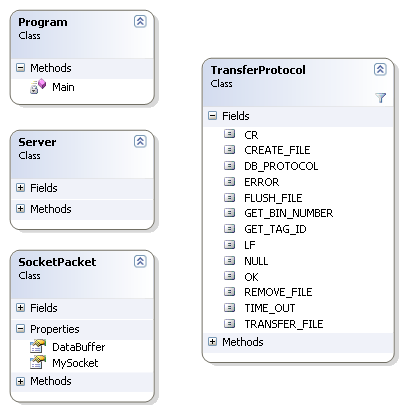
\includegraphics[scale=0.7]{socketClassDiagram}
	\caption{Class diagram of the socket transfer server}
	\label{fig:socketClassDiagram}
\end{figure}

\subsection{Future work}

The socket transfer server can be extended to having files transferring features and security. File transferring protocol is already defined, however not implemented. It could be used to save a profile picture. Security could be used to make safe transfers. Both of above mentioned features are not important. Picture is just additional feature and does not make sense to project. Security only necessary if transferring server will be placed out of the domain, in a public domain. Another important improvement to the socket server protocol, is to enable all the database functions so that the DLL file for connecting to the database that subtask 6 are using will be unecessary. This extension of the protocol will enabling all kinds of clients around the world, using there own programming language to program their client software, to connect to the database and manage the database library.